%%%%%%%%%%%%%%%%%%%%%%%%%%%%%%%%%%%%%%%%%%%%%%%%%%%%%%%%%%%%%%%%%%%%%%%%%%%%%%
%% Lecture 1: Introduction to Machine Learning.
%% Compile with: latexmk -pdf lecture01
%% Handout (overlays collapsed, solutions shown): latexmk -pdf lecture01-handout
%% Speaker notes: add the notes option to \usepackage below.
%%
%% Figures: ../codes/l01_figures.py (run with uv run codes/l01_figures.py).
%% Based on the 2025 slides of Stevan Rudinac and on Lecture 1 of Andreas
%% Mueller's Applied Machine Learning course (Columbia University, 2017).
%%%%%%%%%%%%%%%%%%%%%%%%%%%%%%%%%%%%%%%%%%%%%%%%%%%%%%%%%%%%%%%%%%%%%%%%%%%%%%

% lecture01-handout.tex defines \sibhandout before reading this file.
\ifdefined\sibhandout
  \documentclass[handout,aspectratio=169,t,9pt]{beamer}
  \usepackage[macros,solutions]{siblecture2026}
\else
  \documentclass[aspectratio=169,t,9pt]{beamer}
  \usepackage[macros]{siblecture2026}
\fi

% Everything specific to this course goes here.
\graphicspath{{figures/}{../images/}}
\usepackage{booktabs}
\usetikzlibrary{positioning,arrows.meta}

%%%%%%%%%%%%%%%%%%%%%%%%%%%%%%%%%%%%%%%%%%%%%%%%%%%%%%%%%%%%%%%%%%%%%%%%%%%%%%

\course{Machine Learning with Python}
\coursesubtitle{Minor Amsterdam Data Science and Artificial Intelligence}
\term{Fall 2026}

\lectureno{1}
\title{Introduction to Machine Learning}
\subtitle{What machine learning is, what it can do, and how to think about it}
\author{\c{S}. \.{I}lker Birbil}
\institute{Amsterdam Business School, University of Amsterdam}
\date{October 26, 2026}
\contact{s.i.birbil@uva.nl}

% ============================================================
\begin{document}
% ============================================================

\sibtitleframe

\begin{frame}{Credits}
  \begin{columns}[T,onlytextwidth]
    \begin{column}{0.48\textwidth}
      \begin{sibbox}{Stevan Rudinac (UvA)}
        Taught this course in 2025.  This edition revises his slides.
      \end{sibbox}
    \end{column}
    \begin{column}{0.48\textwidth}
      \begin{sibbox}{Andreas M\"{u}ller (Columbia University)}
        \emph{Applied Machine Learning} (2017), the basis of the 2025
        slides.\\[2pt]
        {\scriptsize\url{https://github.com/amueller/applied_ml_spring_2017}}
      \end{sibbox}
    \end{column}
  \end{columns}

  \vspace{0.6cm}
  \textbf{Textbook.} A.~C. M\"{u}ller and S.~Guido (2016).
  \emph{Introduction to Machine Learning with Python}.  O'Reilly Media.
  Online through the UvA Library.

  \note{Much of the structure, the examples and the notebooks of this course
    come from these two sources.}
\end{frame}

\sibtocframe[Lecture overview]

\begin{frame}{What you should be able to do afterwards}
  \begin{objectives}
    \item Explain what machine learning is.
    \item Tell supervised from unsupervised learning, and classification
          from regression.
    \item Explain why a model must \emph{generalize} to new data.
    \item Ask the right questions before using machine learning at all.
  \end{objectives}
\end{frame}

% ==================================================================
\section{About This Course}
% ==================================================================

\begin{frame}{Who we are}
  \vspace{0.3cm}
  \begin{columns}[T,onlytextwidth]
    \begin{column}{0.48\textwidth}
      \centering
      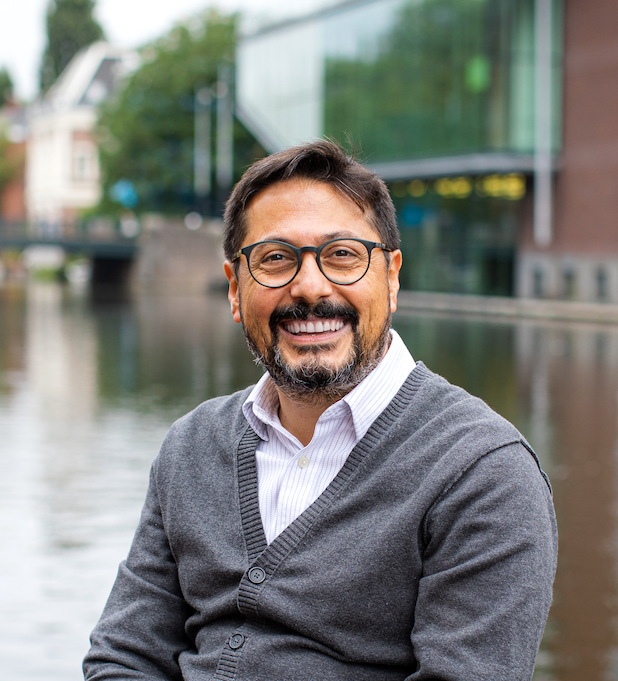
\includegraphics[height=3.0cm]{S_IlkerBirbil.png}

      \vspace{0.3cm}
      \textbf{\c{S}. \.{I}lker Birbil}\\
      Lectures\\
      \href{mailto:s.i.birbil@uva.nl}{\texttt{s.i.birbil@uva.nl}}
    \end{column}
    \begin{column}{0.48\textwidth}
      \centering
      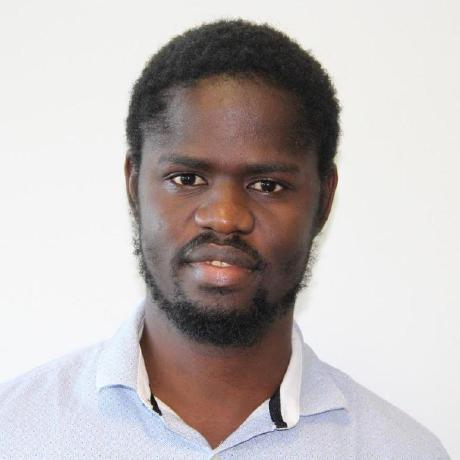
\includegraphics[height=3.0cm]{DiadieSow.jpeg}

      \vspace{0.3cm}
      \textbf{Diadi\'{e} Sow}\\
      Laptop labs\\
      \href{mailto:d.sow@uva.nl}{\texttt{d.sow@uva.nl}}
    \end{column}
  \end{columns}

  \note{Questions about the lectures and the exam go to the lecturer;
    questions about the labs and the programming assignments go to the
    tutor.}
\end{frame}

\begin{frame}{When and where}
  \begin{columns}[T,onlytextwidth]
    \begin{column}{0.56\textwidth}
      \begin{tabular}{@{}lll@{}}
        \toprule
        \textbf{Session} & \textbf{Time} & \textbf{Room} \\
        \midrule
        Lecture, Monday      & 11:00--12:45 & REC A2.09 \\
        Lecture, Tuesday     & 15:00--16:45 & REC A2.11 \\
        Laptop lab, Thursday & 09:00, 11:00 or 15:00 & REC JKTB.20 \\
        \bottomrule
      \end{tabular}

      \vspace{0.4cm}
      \begin{itemize}
        \item October 26 -- December 10
        \item The three labs are identical: attend \highlight{one}.
      \end{itemize}
    \end{column}
    \begin{column}{0.40\textwidth}
      \begin{sibbox}{Written exam}
        Thursday, December 17, 19:00--21:00\\
        World Fashion Center, Westhal
      \end{sibbox}
    \end{column}
  \end{columns}

  \vfill
  \muted{Check the UvA timetable regularly: times and rooms may change.}

  \note{Each lecture has two 45-minute sessions with a break.  Each lab
    lasts 1h45.}
\end{frame}

\begin{frame}{How you are assessed}
  \begin{columns}[T,onlytextwidth]
    \begin{column}{0.48\textwidth}
      \begin{tabular}{@{}lr@{}}
        \toprule
        Individual programming assignments & 20\% \\
        Group project                      & 20\% \\
        Written exam (2 hours)             & 60\% \\
        \bottomrule
      \end{tabular}
    \end{column}
    \begin{column}{0.48\textwidth}
      \begin{keypoint}{To pass}
        Exam $\ge 5.5$ \textbf{and} weighted average $\ge 5.5$.
      \end{keypoint}
    \end{column}
  \end{columns}

  \vfill
  \muted{Resit: only the exam.  Assignment and project grades stay valid
  within the academic year.}
\end{frame}

\begin{frame}{What you need}
  \begin{itemize}
    \item \textbf{Textbook:} M\"{u}ller and Guido (2016), online through the
          UvA Library
    \item \textbf{Software:} Python, installed through Anaconda
    \item \textbf{Background:} no machine learning; high-school mathematics
          and a first statistics course
  \end{itemize}

  \vfill
  \begin{takeaway}
    Lectures: \emph{what} a method does and \emph{when} to use it.
    Labs: \emph{how} to run it in Python.
  \end{takeaway}

  \note{Some programming experience helps; the labs build it up.  Each
    lecture names the relevant chapter of the book.}
\end{frame}

% ==================================================================
\section{What Is Machine Learning?}
% ==================================================================

\begin{frame}{Machine learning}
  \vspace{0.4cm}
  \begin{definition}[Machine learning]
    Programs that \highlight{learn a rule from examples} and use it on
    \highlight{new} observations.
  \end{definition}

  \vspace{0.6cm}
  \begin{itemize}
    \item Input: a dataset.  Output: a \emph{model}.
    \item Close to statistics and optimization, but focused on
          \keyword{prediction}.
  \end{itemize}

  \note{Mitchell (1997): a program learns if its performance on a task
    improves with experience.  Spam: the task is flagging spam, the
    performance is the share classified correctly, the experience is
    e-mails that users marked as spam.}
\end{frame}

\begin{frame}{Writing rules versus learning rules}
  \begin{columns}[T,onlytextwidth]
    \begin{column}{0.48\textwidth}
      \begin{sibbox}{Traditional programming}
        A person writes the rules:\\
        ``\emph{free money} in the subject $\Rightarrow$ spam''
      \end{sibbox}
    \end{column}
    \begin{column}{0.48\textwidth}
      \begin{sibbox}{Machine learning}
        A person collects examples:\\
        thousands of e-mails labeled \emph{spam} or \emph{not spam}
      \end{sibbox}
    \end{column}
  \end{columns}

  \vspace{1.0cm}
  \centering
  \begin{tikzpicture}[
      box/.style={draw=sib@mute,fill=sib@panel,rounded corners,
                  minimum height=0.8cm,minimum width=2.3cm,
                  font=\small,align=center},
      arr/.style={-{Stealth},thick,sib@accent}]
    \node[box] (d) {data\\+ answers};
    \node[box,right=1.2cm of d,fill=sib@boxbg,draw=sib@accent] (l)
      {learning\\algorithm};
    \node[box,right=1.2cm of l] (m) {model};
    \node[box,right=1.2cm of m] (p) {prediction\\for new e-mail};
    \draw[arr] (d) -- (l);
    \draw[arr] (l) -- (m);
    \draw[arr] (m) -- (p);
  \end{tikzpicture}

  \note{Hand-written rules are hard to write and break easily; spammers
    learn to avoid them.  A learned model is updated with new examples when
    the spammers change their tricks.}
\end{frame}

\begin{frame}{Machine learning you used today}
  \begin{columns}[T,onlytextwidth]
    \begin{column}{0.48\textwidth}
      \begin{itemize}
        \item Spam filter
        \item Recommendations for series and songs
        \item Fraud alerts on card payments
      \end{itemize}
    \end{column}
    \begin{column}{0.48\textwidth}
      \begin{itemize}
        \item Face unlock on your phone
        \item Ranking of your social media feed
        \item Translation and chatbots
      \end{itemize}
    \end{column}
  \end{columns}

  \vfill
  \begin{keypoint}{The common pattern}
    A decision made many times, many past examples, a measure of success.
  \end{keypoint}

  \note{Ask the room for more examples before revealing the list.}
\end{frame}

\begin{frame}{Why Python?}
  \begin{columns}[T,onlytextwidth]
    \begin{column}{0.50\textwidth}
      \begin{itemize}
        \item Among the most popular languages (IEEE Spectrum, 2023)
        \item Free and readable
        \item Libraries for every step of an analysis
      \end{itemize}
    \end{column}
    \begin{column}{0.44\textwidth}
      \begin{sibbox}{Libraries in this course}
        \begin{tabular}{@{}ll@{}}
          \texttt{numpy}        & arrays \\
          \texttt{pandas}       & tables \\
          \texttt{matplotlib}   & plots \\
          \texttt{scikit-learn} & machine learning \\
        \end{tabular}
      \end{sibbox}
    \end{column}
  \end{columns}

  \note{The textbook is written around scikit-learn (Pedregosa et al.,
    2011), of which Andreas M\"{u}ller is a core developer.}
\end{frame}

% ==================================================================
\section{Types of Learning}
% ==================================================================

\begin{frame}{Supervised learning}
  \vspace{0.3cm}
  \begin{itemize}
    \item \textbf{Features} $x$: what we know (age, income, words in a review)
    \item \textbf{Label} $y$: what we want to predict (default, price, rating)
  \end{itemize}

  \vspace{0.3cm}
  From examples $(x_{1},y_{1}),\dots,(x_{n},y_{n})$, learn $f$ with
  \begin{equation*}
    f(x) \approx y \quad \text{also for a \highlight{new} } x.
  \end{equation*}

  \vfill
  \begin{keypoint}{Key assumption}
    New data come from the same source as the training data (i.i.d.).
  \end{keypoint}

  \note{In a spreadsheet: one row per example, one column per feature, one
    column with the label.  i.i.d.: independent and identically
    distributed.  A model trained on the students of 2020 may fail on those
    of 2026 if the students have changed.}
\end{frame}

\begin{frame}{Classification and regression}
  \centering
  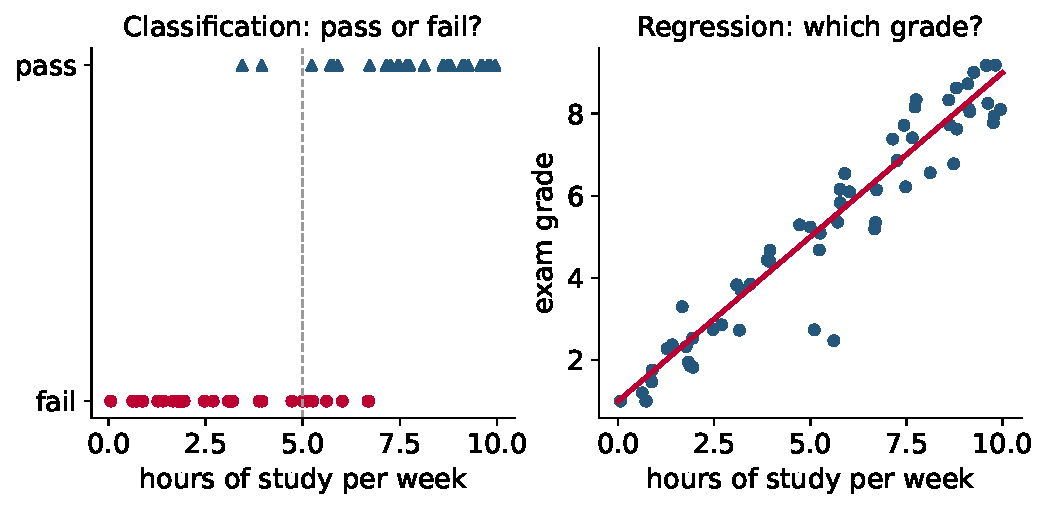
\includegraphics[height=4.0cm]{l01_classification_regression.pdf}

  \vspace{0.3cm}
  \begin{columns}[T,onlytextwidth]
    \begin{column}{0.48\textwidth}
      \textbf{Classification:} the label is a \highlight{category}.
    \end{column}
    \begin{column}{0.48\textwidth}
      \textbf{Regression:} the label is a \highlight{number}.
    \end{column}
  \end{columns}

  \note{Rule of thumb: is the answer a kind (classification) or an amount
    (regression)?}
\end{frame}

\begin{frame}{Supervised learning in business and the social sciences}
  \vspace{0.2cm}
  \begin{tabular}{@{}lll@{}}
    \toprule
    \textbf{Problem} & \textbf{Question} & \textbf{Type} \\
    \midrule
    Credit scoring     & Will the applicant repay?           & classification \\[2pt]
    Customer churn     & Will the subscriber cancel?         & classification \\[2pt]
    Sentiment analysis & Is the review positive or negative? & classification \\[2pt]
    House prices       & What is the apartment worth?        & regression \\
    \bottomrule
  \end{tabular}

  \vfill
  \begin{keypoint}{Where do the labels come from?}
    From the past --- and they are often the costliest part of the data.
  \end{keypoint}

  \note{Features for each: income and payment history; usage and
    complaints; the words of the review; size, neighborhood and year built.}
\end{frame}

\begin{frame}{Unsupervised learning}
  \centering
  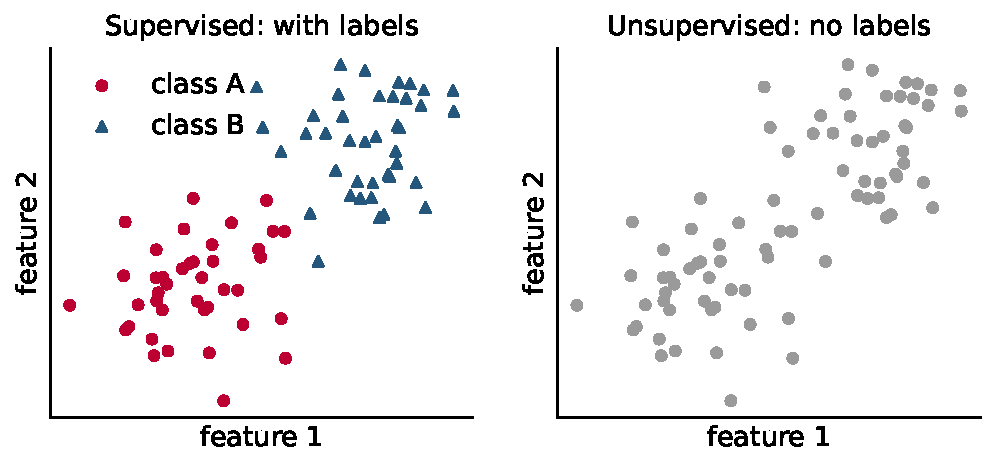
\includegraphics[height=3.8cm]{l01_supervised_unsupervised.pdf}

  \vspace{0.3cm}
  \raggedright
  Only $x$, no $y$: \highlight{find structure}.
  \begin{itemize}
    \item \textbf{Clustering:} customer segments
    \item \textbf{Topic models:} themes in texts (Blei, 2012)
    \item \textbf{Embeddings:} similar items get nearby coordinates
  \end{itemize}
\end{frame}

\begin{frame}{Other kinds of learning}
  \begin{columns}[T,onlytextwidth]
    \begin{column}{0.48\textwidth}
      \begin{sibbox}{Reinforcement learning}
        An agent learns by trial and error from rewards,
        e.g., playing Go (Silver et al., 2016).
      \end{sibbox}
    \end{column}
    \begin{column}{0.48\textwidth}
      \begin{itemize}
        \item Semi-supervised
        \item Self-supervised
        \item Active learning
        \item Forecasting
      \end{itemize}
    \end{column}
  \end{columns}

  \vfill
  \begin{takeaway}
    This course: \textbf{supervised} (Lectures 3--10, 14) and
    \textbf{unsupervised} (Lectures 11--13).
  \end{takeaway}

  \note{Semi-supervised: few labeled, many unlabeled examples.
    Self-supervised: the data provide their own labels, e.g., predict the
    next word; this is how large language models are pre-trained.  Active
    learning: the model asks a person to label the most informative
    examples.  Forecasting: predict a time series such as sales.
    Reinforcement learning is not covered in this course.}
\end{frame}

\begin{frame}{Check your understanding}
  \begin{exercise}[which type of learning?]
    Supervised or unsupervised?  If supervised: classification or
    regression?
    \begin{enumerate}[label=(\alph*),itemsep=1pt,topsep=3pt]
      \item Predict whether a bank customer will default on a loan.
      \item Estimate the selling price of an apartment in Amsterdam.
      \item Group survey respondents who gave similar answers.
      \item Predict next month's revenue of a store.
      \item Decide whether a product review is positive or negative.
      \item Discover the main themes in 10{,}000 open survey comments.
    \end{enumerate}
  \end{exercise}

  \begin{solution}
    (a) Supervised, classification.
    (b) Supervised, regression.
    (c) Unsupervised, clustering.
    (d) Supervised, regression (forecasting).
    (e) Supervised, classification.
    (f) Unsupervised, topic modeling.
  \end{solution}

  \note{Two minutes, alone or with a neighbor, then collect answers by show
    of hands.}
\end{frame}

% ==================================================================
\section{Generalization}
% ==================================================================

\begin{frame}{The first session in one slide}
  \vspace{0.3cm}
  \begin{recap}[Where we are]
    \begin{itemize}
      \item Machine learning learns a rule from examples.
      \item \textbf{Supervised:} features $x$ and label $y$
            (classification or regression).
      \item \textbf{Unsupervised:} only $x$; find structure.
    \end{itemize}
  \end{recap}

  \vspace{0.6cm}
  Now: \highlight{when does a learned rule work}, and \highlight{when is it
  worth building}?
\end{frame}

\begin{frame}{Generalization}
  \vspace{0.3cm}
  \begin{definition}[Generalization]
    A model \emph{generalizes} if it predicts well on \highlight{new} data.
  \end{definition}

  \vspace{0.5cm}
  \begin{itemize}
    \item Memorizing the training data is easy --- and useless.
    \item So we keep a \textbf{test set} aside (Lecture~3).
  \end{itemize}

  \note{Analogy: a student who memorizes last year's exam answers scores
    perfectly on last year's exam and poorly on this year's.  A student who
    understands the material does well on both.}
\end{frame}

\begin{frame}{Too simple, about right, too complex}
  \centering
  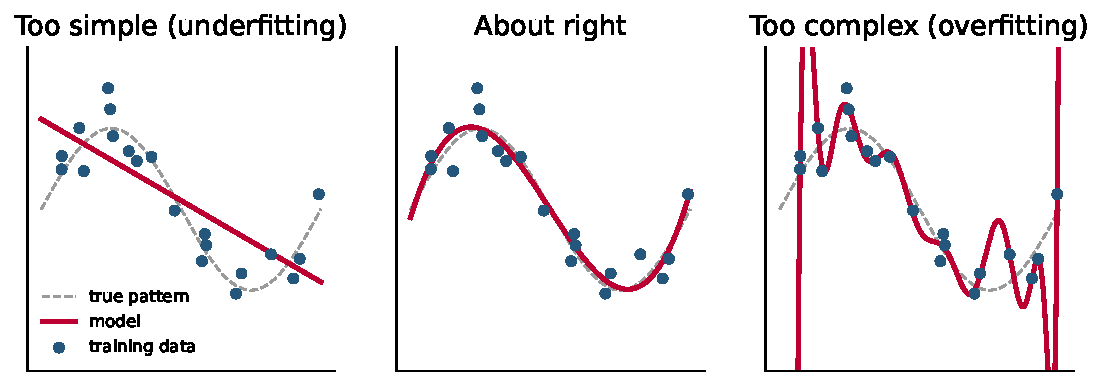
\includegraphics[height=4.0cm]{l01_fitting.pdf}

  \vspace{0.4cm}
  \begin{columns}[T,onlytextwidth]
    \begin{column}{0.32\textwidth}
      \centering\textbf{Underfitting}\\ wrong everywhere
    \end{column}
    \begin{column}{0.32\textwidth}
      \centering\textbf{Good fit}\\ pattern, not noise
    \end{column}
    \begin{column}{0.32\textwidth}
      \centering\textbf{Overfitting}\\ perfect on training data,\\
      poor on new data
    \end{column}
  \end{columns}

  \note{Choosing the right complexity, model selection, is a recurring
    theme of the course.}
\end{frame}

\begin{frame}{Machine learning and statistics}
  \begin{columns}[T,onlytextwidth]
    \begin{column}{0.48\textwidth}
      \begin{sibbox}{Classical statistics}
        \begin{itemize}
          \item Model first
          \item Inference: does education affect income?
        \end{itemize}
      \end{sibbox}
    \end{column}
    \begin{column}{0.48\textwidth}
      \begin{sibbox}{Machine learning}
        \begin{itemize}
          \item Data first
          \item Prediction: what will this person earn?
        \end{itemize}
      \end{sibbox}
    \end{column}
  \end{columns}

  \vfill
  \begin{takeaway}
    Shared methods, different questions: ``two cultures'' (Breiman, 2001).
  \end{takeaway}

  \note{Linear regression appears in both.  Many students know the first
    culture from their statistics courses; this course adds the second, in
    which generalization is checked directly on held-out data.}
\end{frame}

% ==================================================================
\section{Machine Learning in Practice}
% ==================================================================

\begin{frame}{Case study: citizen reports in Amsterdam}
  \begin{columns}[T,onlytextwidth]
    \begin{column}{0.52\textwidth}
      \begin{itemize}
        \item Residents report problems in public space: waste, street
              lights, traffic.
        \item More than 170{,}000 reports per year
              (Rudinac, 2025 lecture slides).
        \item \textbf{Task:} predict the category, to route each report
              to the right department.
      \end{itemize}
    \end{column}
    \begin{column}{0.44\textwidth}
      \begin{sibbox}{Features of one report}
        location \quad text \quad time \quad photo
      \end{sibbox}
    \end{column}
  \end{columns}

  \vfill
  \muted{Sukel, Rudinac and Worring (2019), UvA with the City of Amsterdam.}

  \note{This is supervised classification.  The labels are the categories
    that city staff assigned to past reports.}
\end{frame}

\begin{frame}{What the case study teaches}
  \vspace{0.3cm}
  \begin{keypoint}{Ask of any application}
    \begin{enumerate}
      \item What is the \textbf{decision}?
      \item Where do the \textbf{labels} come from?
      \item What are the \textbf{features}?
      \item What does a \textbf{mistake} cost?
      \item Who \textbf{checks} the model?
    \end{enumerate}
  \end{keypoint}

  \note{For the case: route reports faster; staff categories from past
    years; text, photos, places and times, each turned into features
    (Lectures 6--7); a wrongly routed report is delayed, and some mistakes
    are worse than others (Lectures 9--10); staff correct the predicted
    category, and the corrections become new labels.}
\end{frame}

\begin{frame}{Should you use machine learning at all?}
  \begin{columns}[T,onlytextwidth]
    \begin{column}{0.48\textwidth}
      \begin{itemize}
        \item Data-driven: \textbf{yes}.
        \item Machine learning first: \textbf{no}.
        \item What is the \highlight{baseline}?
        \item What is the \highlight{benefit}?
      \end{itemize}
    \end{column}
    \begin{column}{0.48\textwidth}
      \begin{example}[A closing sale (M\"{u}ller, 2017)]
        A store e-mails its customers about its final sale.  Predict who
        responds?  No: just e-mail everybody.
      \end{example}
    \end{column}
  \end{columns}

  \note{Machine learning systems are complex and fragile: they depend on
    changing data pipelines, are hard to debug, and must be maintained
    (Sculley et al., 2015).  In the example there is no next campaign to
    optimize, so the baseline is the best decision.}
\end{frame}

\begin{frame}{Measure what matters}
  \vspace{0.3cm}
  \begin{itemize}
    \item Only the \textbf{ultimate goal} counts: revenue, health, service.
    \item Often we must use a \textbf{substitute} (proxy).
  \end{itemize}

  \vspace{0.4cm}
  \begin{sibbox}{A music service improves its radio feature}
    \textbf{Better proxy:} listening time, returning users.
    \quad \textbf{Worse proxy:} clicks.
  \end{sibbox}

  \note{A more accurate model that does not move the goal is not an
    improvement.  Clicks also rise when users skip songs they dislike.
    Nobody hands you the goal and the measure of success; defining them is
    part of the job.}
\end{frame}

\begin{frame}{Explain the results}
  \vspace{0.3cm}
  \begin{itemize}
    \item A model is used only if people trust it.
    \item Some decisions must be explained: a rejected loan, a flagged tax
          return.
    \item Simple models are easier to explain; complex ones often predict
          better.
  \end{itemize}

  \note{Users also respond to explanations: ``recommended because you
    watched \dots''  Linear models (Lectures 4--5) and small trees
    (Lecture 8) are easy to explain.  This trade-off returns throughout the
    course.}
\end{frame}

\begin{frame}{Ethics: it is in the application}
  \begin{columns}[T,onlytextwidth]
    \begin{column}{0.48\textwidth}
      \begin{sibbox}{Risk scores in US courts}
        Black defendants who did not reoffend were more often labeled
        high risk than white defendants (Angwin et al., 2016).
      \end{sibbox}
    \end{column}
    \begin{column}{0.48\textwidth}
      \begin{sibbox}{Same model, different use}
        Two schools predict underperforming students.  One removes them;
        the other supports them (M\"{u}ller, 2017).
      \end{sibbox}
    \end{column}
  \end{columns}

  \vfill
  \begin{keypoint}{Discuss with your neighbor (1 minute)}
    A model decides on loans.  Who is harmed by a mistake, and who notices?
  \end{keypoint}

  \note{The US risk-score model was commercial and a black box to the
    defendants and the judges.  In the school example the algorithm can be
    identical; the ethics are not.}
\end{frame}

\begin{frame}{Data: free or expensive?}
  \begin{columns}[T,onlytextwidth]
    \begin{column}{0.48\textwidth}
      \begin{sibbox}{Free: observable events}
        Clicks, stock prices, cancellations
      \end{sibbox}
    \end{column}
    \begin{column}{0.48\textwidth}
      \begin{sibbox}{Expensive: expert labels}
        Diagnoses, drug trials, coded survey answers
      \end{sibbox}
    \end{column}
  \end{columns}

  \vfill
  \begin{keypoint}{More data?}
    Worth it if the gain for the goal exceeds the cost.
  \end{keypoint}

  \note{Free labels appear by themselves as time passes; expensive labels
    must be produced by someone, often an expert.  More data from the right
    source usually improves a model.}
\end{frame}

% ==================================================================
\section{The Workflow and the Road Ahead}
% ==================================================================

\begin{frame}{The machine learning workflow}
  \vspace{0.6cm}
  \centering
  \begin{tikzpicture}[
      box/.style={draw=sib@mute,fill=sib@panel,rounded corners,
                  minimum height=1.0cm,text width=1.7cm,
                  font=\scriptsize,align=center},
      arr/.style={-{Stealth},thick,sib@accent}]
    \node[box,fill=sib@boxbg,draw=sib@accent] (g)
      {\textbf{Goal}\\and measure};
    \node[box,right=0.3cm of g] (d) {\textbf{Collect}\\and explore};
    \node[box,right=0.3cm of d] (f) {\textbf{Clean},\\features};
    \node[box,right=0.3cm of f] (m) {\textbf{Train}\\models};
    \node[box,right=0.3cm of m] (e) {\textbf{Evaluate}\\and select};
    \node[box,right=0.3cm of e] (u) {\textbf{Deploy}\\and monitor};
    \foreach \a/\b in {g/d,d/f,f/m,m/e,e/u} \draw[arr] (\a) -- (\b);
    \draw[arr,dashed] (e.south) to[out=-150,in=-30]
      node[below,font=\scriptsize,text=sib@mute] {go back} (f.south);
    \node[font=\scriptsize,text=sib@mute,above=0.05cm of g] {L1};
    \node[font=\scriptsize,text=sib@mute,above=0.05cm of d] {L2};
    \node[font=\scriptsize,text=sib@mute,above=0.05cm of f] {L6--7};
    \node[font=\scriptsize,text=sib@mute,above=0.05cm of m] {L3--8, 14};
    \node[font=\scriptsize,text=sib@mute,above=0.05cm of e] {L3, 9--10};
    \node[font=\scriptsize,text=sib@mute,above=0.05cm of u] {project};
  \end{tikzpicture}

  \vfill
  \begin{takeaway}
    Training is a small part of the work; the goal, the data and the
    evaluation take most of the time.
  \end{takeaway}

  \note{The cornerstones of the course: define the problem and the measure
    of success; prepare data and engineer features; know the strengths and
    weaknesses of algorithms; select and evaluate models soundly.  The
    steps are repeated many times.}
\end{frame}

\begin{frame}{The road ahead}
  \footnotesize
  \begin{tabular}{@{}lll@{}}
    \toprule
    \textbf{Week} & \textbf{Monday} & \textbf{Tuesday} \\
    \midrule
    1 & Oct 26: Introduction              & Oct 27: Visualization \\
    2 & Nov 2: Supervised learning        & Nov 3: Linear regression \\
    3 & Nov 9: Linear classification      & Nov 10: Preprocessing \\
    4 & Nov 16: Imputation, feature selection & Nov 17: Trees and forests \\
    5 & Nov 23: Model evaluation          & Nov 24: Imbalanced data \\
    6 & Nov 30: Clustering                & Dec 1: Evaluating clustering \\
    7 & Dec 7: NMF, outlier detection     & Dec 8: Neural networks \\
    \bottomrule
  \end{tabular}

  \vfill
  \normalsize
  \muted{Labs every Thursday.  Exam: Thursday, December 17.}
\end{frame}

\begin{frame}{Before Thursday: install Python}
  \vspace{0.3cm}
  \begin{enumerate}
    \item Download Anaconda: \url{https://www.anaconda.com/download}
    \item Install with the default settings.
    \item In Jupyter Notebook, run
          \texttt{import sklearn; print(sklearn.\_\_version\_\_)}
  \end{enumerate}

  \vfill
  \begin{takeaway}
    Setup guide: \texttt{python\_setup.pdf} (Stevan Rudinac).
    Bring your laptop to the first lab on October 29.
  \end{takeaway}

  \note{Anaconda includes Python, Jupyter Notebook, numpy, pandas,
    matplotlib and scikit-learn.  If a version number appears, the
    installation works.}
\end{frame}

\begin{frame}{Check your understanding}
  \begin{exercise}[three exam-style questions]
    \begin{enumerate}[itemsep=3pt,topsep=3pt]
      \item Near-perfect on the training data, poor on new data:\\
            A.~underfitting \quad B.~overfitting \quad
            C.~generalization \quad D.~clustering
      \item A closing shop sends one final e-mail about its sale.  It
            should\\
            A.~predict who responds \quad B.~e-mail every customer \quad
            C.~cluster customers \quad D.~collect more data
      \item The machine learning view judges a model by\\
            A.~its parameters \quad B.~its predictions on new data \quad
            C.~its fit to the training data
    \end{enumerate}
  \end{exercise}

  \begin{solution}
    1.~B.  2.~B: there is no future campaign, so the baseline wins.
    3.~B: C would reward overfitting.
  \end{solution}
\end{frame}

\begin{frame}{Where this is going}
  \vspace{0.3cm}
  \begin{takeaway}
    Machine learning learns a rule from examples and is judged on new data.
    First define the goal, the baseline and the cost of a mistake.
  \end{takeaway}

  \vfill
  \begin{comingup}
    Lecture~2 (Tuesday, October 27): visualization with
    \texttt{matplotlib}.
  \end{comingup}

  \vfill
  \textbf{Reading.} M\"{u}ller and Guido (2016), Chapter~1.
\end{frame}

\begin{frame}{References}
  \scriptsize
  \begin{itemize}
    \item Angwin, J., Larson, J., Mattu, S., and Kirchner, L. (2016).
          Machine bias.  \emph{ProPublica}, May 23, 2016.
          \url{https://www.propublica.org/article/machine-bias-risk-assessments-in-criminal-sentencing}
    \item Blei, D.~M. (2012).  Probabilistic topic models.
          \emph{Communications of the ACM}, 55(4), 77--84.
    \item Breiman, L. (2001).  Statistical modeling: The two cultures.
          \emph{Statistical Science}, 16(3), 199--231.
    \item IEEE Spectrum (2023).  The top programming languages 2023.
          \url{https://spectrum.ieee.org/the-top-programming-languages-2023}
    \item Mitchell, T.~M. (1997).  \emph{Machine Learning}.  McGraw-Hill.
    \item M\"{u}ller, A.~C. (2017).  Applied Machine Learning, Lecture 1:
          Introduction.  Columbia University.
          \url{https://github.com/amueller/applied_ml_spring_2017}
    \item M\"{u}ller, A.~C. and Guido, S. (2016).  \emph{Introduction to
          Machine Learning with Python: A Guide for Data Scientists}.
          O'Reilly Media.
    \item Pedregosa, F. et al. (2011).  Scikit-learn: Machine learning in
          Python.  \emph{Journal of Machine Learning Research}, 12,
          2825--2830.
    \item Rudinac, S. (2025).  Machine Learning, Lecture 1: Introduction.
          Lecture slides, University of Amsterdam.
    \item Sculley, D. et al. (2015).  Hidden technical debt in machine
          learning systems.  \emph{Advances in Neural Information
          Processing Systems}, 28.
    \item Silver, D. et al. (2016).  Mastering the game of Go with deep
          neural networks and tree search.  \emph{Nature}, 529, 484--489.
    \item Sukel, M., Rudinac, S., and Worring, M. (2019).  Multimodal
          classification of urban micro-events.  In \emph{Proceedings of
          the 27th ACM International Conference on Multimedia (MM '19)}.
  \end{itemize}
\end{frame}

\end{document}
